% Created 2023-01-12 Πεμ 19:38
% Intended LaTeX compiler: pdflatex
\documentclass[11pt]{article}
\usepackage[utf8]{inputenc}
\usepackage[T1]{fontenc}
\usepackage{graphicx}
\usepackage{longtable}
\usepackage{wrapfig}
\usepackage{rotating}
\usepackage[normalem]{ulem}
\usepackage{amsmath}
\usepackage{amssymb}
\usepackage{capt-of}
\usepackage{hyperref}
\usepackage{booktabs}
\usepackage{import}
\usepackage[LGR, T1]{fontenc}
\usepackage[greek, english]{babel}
\usepackage{alphabeta}
\usepackage{esint}
\usepackage{mathtools}
\usepackage{esdiff}
\usepackage{makeidx}
\usepackage{glossaries}
\usepackage{newfloat}
\usepackage{minted}
\usepackage{chemfig}
\usepackage{svg}
\usepackage[a4paper, margin=3cm]{geometry}
\author{Διονύσης Γιαννάτος}
\date{\today}
\title{Ανάλυση του Block 200 - Παραγωγή Γλυκόζης}
\hypersetup{
 pdfauthor={Διονύσης Γιαννάτος},
 pdftitle={Ανάλυση του Block 200 - Παραγωγή Γλυκόζης},
 pdfkeywords={},
 pdfsubject={},
 pdfcreator={Emacs 28.2 (Org mode 9.5.5)}, 
 pdflang={English}}
\makeatletter
\newcommand{\citeprocitem}[2]{\hyper@linkstart{cite}{citeproc_bib_item_#1}#2\hyper@linkend}
\makeatother

\usepackage[notquote]{hanging}
\begin{document}

\maketitle
\tableofcontents

\renewcommand{\abstractname}{Περίληψη}
\renewcommand{\tablename}{Πίνακας}
\renewcommand{\figurename}{Σχήμα}
\renewcommand\listingscaption{Κώδικας}

\section{Διάγραμμα Ροής και επεξήγηση}
\label{sec:orgc0a70d9}
\begin{figure}[htbp]
\centering
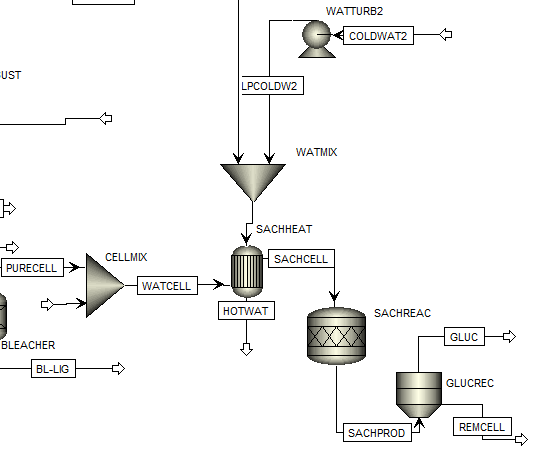
\includegraphics[width=300px]{/home/vidianos/Documents/7o_εξάμηνο/Σχεδιασμός_Ι/Project/git_repo/Final_exam_files/Block_200_-_Παραγωγή_Γλυκόζης/2023-01-10_18-39-54_screenshot.png}
\caption{Διάγραμμα Ροής του block 200}
\end{figure}

Στην παραπάνω εικόνα είναι εμφανής η διεργασία ψύξης και σακχαροποίησης
της κυτταρίνης σε γλυκόζη. Ο εναλλάκτης θερμότητας ψύχει την κυτταρίνη
στους 50 βαθμούς Κελσίου από τους 200 που προκύπτει από την διεργασία
έκρηξης ατμού, ο οποίος αποτυπώνεται στο Block 100. Αξίζει να αναφερθεί πως στην πραγματικότητα, η ψύξη αυτή πρέπει να γίνει μετά την έκρηξη ατμού στο block 100. Όμως, αυτό διαπιστώθηκε αργότερα για αυτό δεν έχει αποτυπωθεί ακόμη στο Aspen.

Έπειτα, η κυτταρίνη τροφοδοτείται σε έναν αντιδραστήρα, ο οποίος αντιπροσωπεύεται στο Aspen ως αντιδραστήρας RYield, και ύστερα τροφοδοτείται σε φυγόκεντρο για τον
διαχωρισμό της στερεής κυτταρίνης από το διάλυμα γλυκόζης, το οποίο
κατευθύνεται στο Block 400 για την παραγωγή γλυκερόλης.

\section{Σχεδιαστικές Επιλογές}
\label{sec:org30421d4}
Η κύρια σχεδιαστική επιλογή σε αυτό το block είναι η επιλογή του είδους
αντιδραστήρα και των συνθηκών λειτουργίας του. Για τις συνθήκες
λειτουργίας, επιλέχθηκε ο αντιδραστήρας αυτός να λειτουργεί στους 50
βαθμούς Κελσίου και σε ατμοσφαιρική πίεση, εφόσον, σύμφωνα με την
βιβλιογραφία, αυτές οι συνθήκες εξασφαλίζουν την βέλτιστη λειτουργία των
κυτταρολυτικών ενζύμων. Σε αντίθεση με κλασσικές χημικές διεργασίες, οι
οποίες μπορούν να γίνουν σε διάφορες θερμοκρασίες, οι ενζυμικές
αντιδράσεις απενεργοποιούνται σε μεγάλες θερμοκρασίες λόγω μετουσίωσης
του ενζύμου. Άρα, η καμπύλη ρυθμού της αντίδρασης περιέχει μέγιστο γι'
αυτή την θερμοκρασία.

Στην πράξη, αυτή η αντίδραση είναι μια διφασική αντίδραση μεταξύ της
στερεής φάσης, δηλαδή της κυτταρίνης, και των κυτταρολυτικών ενζύμων που
βρίσκονται σε υδατική φάση, αποκλείοντας την χρήση ακινητοποιημένων
ενζύμων. Το βέλτιστο είδος αντιδραστήρα θα ήταν ένας αντιδραστήρας
είδους CSTR με μεμβράνη που επιτρέπει την έξοδο των προϊόντων της
σακχαροποίησης, αλλά όχι στα ίδια τα ένζυμα, ώστε να μειωθεί το κόστος
των ενζύμων, και να αποφευχθεί η αναστολή του ενζύμου λόγω του
προϊόντος.

Βέβαια, λόγω της περιπλοκότητας της αντίδρασης αυτής και καθώς δεν είναι από τις κύριες αντιδράσεις της διεργασίας, αυτή δεν προσομοιώθηκε ως RCSTR αλλά ως RStoic όπως θα αναφερθεί και παρακάτω.

\section{Υπολογισμοί}
\label{sec:orgc91d3d9}
Σύμφωνα με την προσομοίωση στο Block 100, εξέρχονται 6900 kg/hr
κυτταρίνης από τον αντιδραστήρα έκρηξης ατμού. Στον αντιδραστήρα
ενζυμικής σακχαροποίησης, με χρόνο παραμονής 72 ώρες και τις προαναφερόμενες συνθήκες, επιτυγχάνεται μετατροπή 0.54 αν η τροφοδοσία γίνει bleached και απομακρυνθεί όλη η λιγνίνη που έχει \textsuperscript{\citeprocitem{1}{1}} . Άρα, στην έξοδο
υπάρχουν 4140 kg/hr γλυκόζη και 3174 kg/hr κυτταρίνη, η οποία διαχωρίζεται
μέσω φυγοκέντρησης και οδηγείται πίσω στον αντιδραστήρα για
σακχαροποίηση ενώ το υδατικό διάλυμα της γλυκόζης οδηγείται στο block 400 για παραγωγή γλυκερόλης.

\section{Προσομοιώσεις στο Aspen}
\label{sec:orga6b1221}
Για την προσομοίωση της ενζυμικής σακχαροποίησης, χρησιμοποιήθηκε αρχικά αντιδραστήρας είδους RYield. Η προσομοίωση της πραγματικής στοιχειομετρίας και κινητικής της αντίδρασης είναι αρκετά περίπλοκη για αυτό έγινε αυτό με τα yields της βιβλιογραφίας \textsuperscript{\citeprocitem{1}{1}}. Το αίτιο για την χρήση αντιδραστήρα RYield είναι πως η αντίδραση της κυτταρίνης σε γλυκόζη είναι μια αντίδραση αποπολυμερισμού, χωρίς να είναι γνωστό το μήκος της αλυσίδας. Παράλληλα, είναι μια αντίδραση χωρίς καθορισμένη στοιχειομετρική αναλογία, και τέλος, είναι μία αρκετά περίπλοκη αντίδραση που περιέχει 3 στάδια, άρα και 3 αντιδράσεις.

Βέβαια, καταλήξαμε σε μία πιό απλοποιημένη προσέγγιση όπου η κυτταρίνη ορίστηκε ως στερεό με μοριακό τύπο μία δομική μονάδα κυτταρίνης \textsuperscript{\citeprocitem{2}{2}} η οποία αντιδρά με στοιχειομετρία 1-1 με νερό παράγοντας γλυκόζη. Αυτή η αντίδραση προσομοιώθηκε εν τέλει σε RStoic για να μην μπλέξει η αρκετά περίπλοκη της κινητική με μετατροπή αυτή που υπάρχει στην βιβλιογραφία \textsuperscript{\citeprocitem{1}{1}} .

Η ψύξη του ρεύματος έγινε με νερό ψύξης σε χαμηλή πίεση, ορίζοντας ότι η έξοδος του θερμού ρεύματος (κυτταρίνη) πρέπει να είναι 50 \(^oC\). Τέλος, ο διαχωρισμός της κυτταρίνης έγινε με ένα CFuge με το μοντέλο Decanter.

\section{Βιβλιογραφία}
\label{sec:orgbc496c1}
\hypertarget{citeproc_bib_item_1}{(1) Fernandez-Bolanos, J.; Felizon, B.; Heredia, A.; Rodriguez, R.; Guillen, R.; Jimenez, A. Steam-Explosion of Olive Stones: Hemicellulose Solubilization and Enhancement of Enzymatic Hydrolysis of Cellulose. \textit{Bioresource technology} \textbf{2001}, \textit{79} (1), 53–61. \url{https://doi.org/10.1016/S0960-8524(01)00015-3}.}

\hypertarget{citeproc_bib_item_2}{(2) Wooley, R. J.; Putsche, V. Development of an ASPEN PLUS Physical Property Database for Biofuels Components. \textbf{1996}, 36.}
\end{document}